% explanations http://www.math.umbc.edu/~rouben/beamer/
\documentclass{beamer}

\usepackage{style/beamertheme_amsterdam}
% \renewcommand{\labelitemi}{$\vcenter{\hbox{\tiny$\bullet$}}$}
\beamertemplatenavigationsymbolsempty
\usepackage{natbib}
\usepackage{tikz}
\usepackage{pbox}
\usepackage{listings}
\lstset{language=Java} 
\usepackage{mdframed}
\mdfdefinestyle{IndexFrame}{%
    linecolor=blue,
    outerlinewidth=2pt,
    roundcorner=20pt,
    innertopmargin=\baselineskip,
    innerbottommargin=\baselineskip,
    innerrightmargin=20pt,
    innerleftmargin=20pt
    innermargin=10pt
    }

\title{Designing an Index for ZooDB}
%\subtitle{}
\author{Jonas Nick \& Bogdan Vancea}
\begin{document}
  \frame{\titlepage}
  \begin{frame}
    \frametitle{Outline}
    \tableofcontents[hideallsubsections]
  \end{frame}

  \begin{section}{What is...?}
    \begin{frame}
      \frametitle{ZooDB}
      \begin{itemize}
        \item an open source object database written in Java
        \item JDO standard compliant
        \item 4 times faster than competitor db4o
        \item \url{zoodb.org}
      \end{itemize}

    \end{frame}
    \begin{frame}
      \frametitle{Database Index}
      \begin{block}{}
          Key-Value datastructure that allows ordered iteration.
      \end{block}
      \vspace{1em}
      % Example: \lstinline|ZooJdoHelper.createIndex(pm, Person.class, "name", false);|
      \pause
      Example: \\
      \texttt{ZooJdoHelper.createIndex(pm, Person.class, "name", false);}
      \pause
      \begin{align*}
      \fbox{\parbox[t][3em][c]{0.29\textwidth}{Attribute \\ Value $\rightarrow$ Object-ID} }
      \end{align*}
      \pause
      \begin{center}
      \fbox{\parbox[t][3em][c]{0.29\textwidth}{OID \\ Object-ID $\rightarrow$ Diskpos} }
      \fbox{\parbox[t][3em][c]{0.29\textwidth}{FSM \\ Page-ID $\rightarrow$ TxID} }
      \end{center}
    \end{frame}
    \begin{frame}
      \frametitle{B+ Tree}
      \begin{itemize}
        \item node fills one disk page
        \item inner node contains keys and children pointer, leaves contain keys and values
        \item key unique vs. key-value unique
      \end{itemize}
    \end{frame}
    \begin{frame}
      \frametitle{Example: insert}
    \end{frame}
  \end{section}

  \begin{section}{The new Index Implementation}
    3908 loc + 2665 loc of test
    \begin{frame}
      \frametitle{Goals}
        \begin{itemize}
          \item fast B+ tree index
          \item buffer manager to allow caching
          \item prefix sharing
        \end{itemize}
    \end{frame}
    \begin{frame}
      \frametitle{Challenges - General}
        \begin{itemize}
          \item edge cases
          \item runtime dominated by disk access
          \begin{itemize}
            \item change nodes infrequently
            \item fewer nodes is better
          \end{itemize}
          \item only parent to child pointer
          \item determine best when its time to split/redistribute
          \item key unique vs. key-value unique
          \item buffer manager lookup takes time 
          \item prefix-sharing encoding/decoding takes time
          \item prefix-sharing rebalancing takes time
          \item general optimizations
            \begin{itemize}
              \item avoid polymorphism
              \item bit-level operations
            \end{itemize}
        \end{itemize}
    \end{frame}
    
    % \begin{frame}
    %   \frametitle{Buffer Manager}
    % \end{frame}
    \begin{frame}
      \frametitle{Prefix Sharing}
      \setbeamercovered{invisible}
      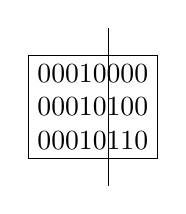
\begin{tikzpicture}
        \node[draw,align=left] at (0,2) {00010000\\ 00010100\\ 00010110};
        \onslide<2->{\draw (0.2,1) -- (0.2,3);}
      \end{tikzpicture}
      \pause
      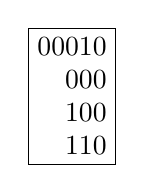
\begin{tikzpicture}
        \onslide<3->{\node[draw,align=right] at (0,2) {00010\\ 000\\100\\110};}
      \end{tikzpicture}
    \end{frame}
    \begin{frame}
      \frametitle{Prefix Sharing}
      \begin{block} {Normal storage of a list of words}
      [skydive, skyline, skyscraper] 
      \end{block}
      \begin{block} {Can exploit common prefix}
      sky + [dive, line, scaper]
      \end{block}
      This trick can also be applied on bit srings
    \end{frame}
    \begin{frame}
        \frametitle{Challenges - Prefix Sharing}
        \begin{itemize}
            \item variable number of key-value entries per page
            \item prefix determines
            \begin{itemize}
                \item if 2 nodes can be merged without overflow
                \item the number of entries that can be redistributed from one node to the other
            \end{itemize}
        \end{itemize}    
    \end{frame}
    \begin{frame}
      \frametitle{Our B+ Tree}
      \begin{itemize}
        \item 64 bit keys and 64 bit values
        \item key unique and key non-unique variants
        \item keys encoded based on common bit prefix
      \end{itemize}
    \end{frame}
    \begin{frame}
        \frametitle{Class Diagram}
        Make it and add it here    
    \end{frame}
    \begin{frame}
        \frametitle{Operations}
        \begin{itemize}
        \item Search - Similar to normal B+ Tree
        \item Insert overflow
            \begin{itemize}
            \item attempt to redistribute values to left sibling before creating a new node
            \end{itemize}
        \item Delete underflow
            \begin{itemize}
            \item check if possible to merge with left or right neighbour
            \item check if possible to split current node between left and right
            \item redistribute from left or right
            \end{itemize}
        \end{itemize}
    \end{frame}
  \end{section}

  \begin{section}{Benchmarks}
    \begin{frame}
      \frametitle{Fine grained}
        \begin{itemize}
          \item insert, remove, write
          \item duration, number of nodes
          \item prefix-sharing vs. no prefix-sharing
        \end{itemize}
    \end{frame}
    \begin{frame}
      \frametitle{Whole system}
        \begin{itemize}
          \item test harness
          \item partial PolePosition benchmark
          \item StackOverflow
        \end{itemize}
    \end{frame}
  \end{section}

  \begin{frame}
    \frametitle{Summary}
      \begin{itemize}
        \item ...
      \end{itemize}
  \end{frame}

  \begin{frame}
    \frametitle{Outlook}
      \begin{itemize}
        \item ...
      \end{itemize}
  \end{frame}

\end{document}
